\documentclass[11pt,a4paper]{article}

% Packages
\usepackage[utf8]{inputenc}
\usepackage[T1]{fontenc}
\usepackage{amsmath,amssymb,amsfonts}
\usepackage{graphicx}
\usepackage{booktabs}
\usepackage{longtable}
\usepackage{array}
\usepackage{multirow}
\usepackage{geometry}
\usepackage{hyperref}
\usepackage{xcolor}
\usepackage{listings}
\usepackage{enumitem}
\usepackage{tikz}
\usetikzlibrary{shapes,arrows,positioning,calc}

\geometry{margin=1in}

% Colors
\definecolor{SIRblue}{RGB}{31,119,180}
\definecolor{SIRorange}{RGB}{255,127,14}
\definecolor{SIRgreen}{RGB}{44,160,44}
\definecolor{SIRred}{RGB}{214,39,40}
\definecolor{codegreen}{rgb}{0,0.6,0}
\definecolor{codegray}{rgb}{0.5,0.5,0.5}
\definecolor{codepurple}{rgb}{0.58,0,0.82}
\definecolor{backcolour}{rgb}{0.95,0.95,0.92}

% Listings style
\lstdefinestyle{mystyle}{
    backgroundcolor=\color{backcolour},   
    commentstyle=\color{codegreen},
    keywordstyle=\color{codepurple},
    numberstyle=\tiny\color{codegray},
    stringstyle=\color{SIRorange},
    basicstyle=\ttfamily\footnotesize,
    breakatwhitespace=false,         
    breaklines=true,                 
    captionpos=b,                    
    keepspaces=true,                 
    numbers=left,                    
    numbersep=5pt,                  
    showspaces=false,                
    showstringspaces=false,
    showtabs=false,                  
    tabsize=2
}
\lstset{style=mystyle}

% Title
\title{\textbf{EpiRecipe: A Constraint-Based Pipeline for Generating\\Diverse Compartmental Epidemic Models}\\[0.5em]
\large Technical Report v3.0}
\author{CAPE Project}
\date{November 2025}

\begin{document}

\maketitle

\begin{abstract}
This technical report documents \textbf{EpiRecipe}, an enhanced pipeline for generating diverse, epidemiologically valid compartmental models. The system features constraint-based compartment selection, automatic transition construction, hierarchical parameter sampling, and comprehensive model validation. EpiRecipe supports 12 compartment types, over 20 transition dynamics, and multiple population stratification schemes. The pipeline achieves 100\% valid model generation through careful constraint enforcement and validation rules.
\end{abstract}

\tableofcontents
\newpage

%==============================================================================
\section{Introduction}
%==============================================================================

EpiRecipe is a comprehensive framework for generating diverse compartmental epidemic models. Traditional approaches often rely on hand-crafted models (SIR, SEIR, etc.), limiting the diversity of generated epidemics for training machine learning models. EpiRecipe addresses this by providing:

\begin{enumerate}[itemsep=0pt]
    \item \textbf{Constraint-based compartment selection}: Automatically resolves dependencies between compartments
    \item \textbf{Automatic transition construction}: Builds valid transition networks based on selected compartments
    \item \textbf{Hierarchical parameter sampling}: Samples epidemiologically consistent parameters
    \item \textbf{Model validation}: Ensures population conservation, no dead-ends, and positive $R_0$
    \item \textbf{Population stratification}: First-class support for age/risk group modeling
\end{enumerate}

\subsection{System Architecture}

The EpiRecipe pipeline consists of six stages:

\begin{center}
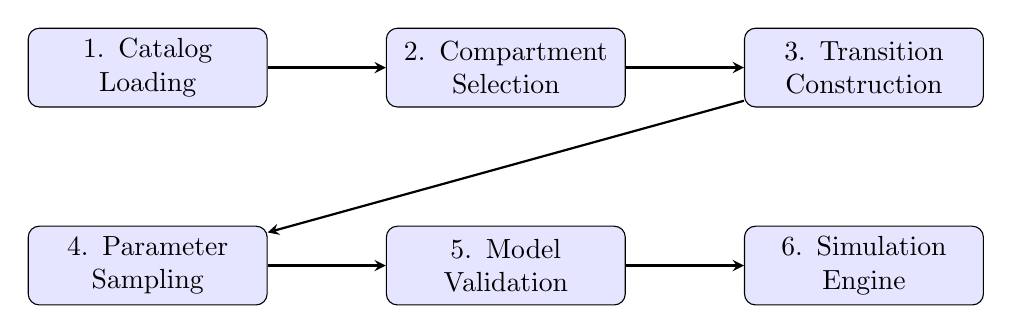
\begin{tikzpicture}[node distance=1.5cm, auto,
    block/.style={rectangle, draw, fill=blue!10, text width=2.8cm, text centered, rounded corners, minimum height=1cm},
    arrow/.style={->, thick, >=stealth}]
    
    \node[block] (catalog) {1. Catalog\\Loading};
    \node[block, right=of catalog] (select) {2. Compartment\\Selection};
    \node[block, right=of select] (trans) {3. Transition\\Construction};
    \node[block, below=of catalog] (params) {4. Parameter\\Sampling};
    \node[block, right=of params] (valid) {5. Model\\Validation};
    \node[block, right=of valid] (sim) {6. Simulation\\Engine};
    
    \draw[arrow] (catalog) -- (select);
    \draw[arrow] (select) -- (trans);
    \draw[arrow] (trans) -- (params);
    \draw[arrow] (params) -- (valid);
    \draw[arrow] (valid) -- (sim);
\end{tikzpicture}
\end{center}

%==============================================================================
\section{Compartment Catalog}
%==============================================================================

EpiRecipe's catalog (v3.0.0) defines 12 epidemiological compartments, each with specific roles, conservation properties, and dependency constraints.

\subsection{Compartment Overview}

\begin{longtable}{@{}llccp{6cm}@{}}
\toprule
\textbf{Symbol} & \textbf{Type} & \textbf{Required} & \textbf{Role} & \textbf{Description} \\
\midrule
\endfirsthead
\toprule
\textbf{Symbol} & \textbf{Type} & \textbf{Required} & \textbf{Role} & \textbf{Description} \\
\midrule
\endhead
\bottomrule
\endfoot

\textbf{S} & susceptible & \checkmark & source & Susceptible individuals who can contract the disease \\
\textbf{I} & infectious & \checkmark & infectious & Infectious individuals who can transmit the disease \\
\textbf{E} & latent & -- & intermediate & Exposed (infected but not yet infectious) individuals \\
\textbf{R} & removed & -- & sink & Recovered or removed individuals with immunity \\
\textbf{A} & infectious & -- & infectious & Asymptomatic infectious individuals \\
\textbf{H} & severe & -- & severe & Hospitalized individuals \\
\textbf{D} & terminal & -- & terminal\_sink & Deceased individuals \\
\textbf{V} & protected & -- & protected & Vaccinated individuals \\
\textbf{Q} & isolated & -- & isolated & Quarantined individuals under isolation \\
\textbf{W} & reservoir & -- & reservoir & Environmental reservoir (water, surfaces) \\
\textbf{C} & chronic & -- & infectious & Chronic carriers with prolonged infectiousness \\
\textbf{P} & protected & -- & protected & Protected individuals (e.g., prophylaxis) \\
\end{longtable}

\subsection{Compartment Dependencies}

Several compartments have constraints requiring other compartments to exist:

\begin{itemize}[itemsep=0pt]
    \item \textbf{E} (Exposed): Requires inflow from S, outflow to I or A
    \item \textbf{A} (Asymptomatic): Requires compartment E (branching from latent)
    \item \textbf{H} (Hospitalized): Requires inflow from I
    \item \textbf{V} (Vaccinated): Requires inflow from S
    \item \textbf{Q} (Quarantined): Requires inflow from I or E
    \item \textbf{W} (Environment): Requires inflow from I or A
    \item \textbf{C} (Chronic): Requires inflow from I
    \item \textbf{P} (Protected): Requires inflow from S
\end{itemize}

\subsection{Conservation Properties}

\begin{itemize}[itemsep=0pt]
    \item \textbf{Conserved compartments}: S, I, E, R, A, H, V, Q, C, P
    \item \textbf{Non-conserved compartments}: D (death), W (environmental reservoir)
    \item \textbf{Conservation rule}: $S + E + I + A + R + H + V + Q + C + P = N - D$
\end{itemize}

%==============================================================================
\section{Transition Dynamics}
%==============================================================================

The catalog defines comprehensive transition dynamics with multiple variants for each type. Transitions are automatically constructed based on selected compartments.

\subsection{Infection Dynamics}

The infection process supports 7 variants:

\begin{longtable}{@{}lp{5cm}p{5cm}@{}}
\toprule
\textbf{Variant} & \textbf{Equation} & \textbf{Requirements} \\
\midrule
\endfirsthead
\toprule
\textbf{Variant} & \textbf{Equation} & \textbf{Requirements} \\
\midrule
\endhead
\bottomrule
\endfoot

mass\_action & $\beta \cdot S \cdot I / N$ & None (default) \\
with\_asymptomatic & $\beta \cdot S \cdot (I + \epsilon A) / N$ & Requires A \\
with\_chronic & $\beta \cdot S \cdot (I + \delta_C C) / N$ & Requires C \\
environmental & $\beta_W \cdot S \cdot W / (K + W)$ & Requires W \\
combined\_environmental & $\beta \cdot S \cdot (I + \rho W) / N$ & Requires W \\
hospital\_nosocomial & $\beta \cdot S \cdot (I + \theta H) / N$ & Requires H \\
saturating & $\beta \cdot S \cdot I / (N \cdot (1 + \alpha I))$ & None \\
\end{longtable}

\subsection{Latent Progression (E $\rightarrow$ I/A)}

\begin{longtable}{@{}lp{5cm}p{5cm}@{}}
\toprule
\textbf{Variant} & \textbf{Equation} & \textbf{Description} \\
\midrule
simple & $\sigma \cdot E \rightarrow I$ & Direct progression to infectious \\
branching & $\sigma \cdot E \rightarrow \{p_{sym} \cdot I, (1-p_{sym}) \cdot A\}$ & Split to symptomatic/asymptomatic \\
\bottomrule
\end{longtable}

\subsection{Recovery Dynamics}

\begin{longtable}{@{}lp{5cm}p{5cm}@{}}
\toprule
\textbf{Variant} & \textbf{Equation} & \textbf{Description} \\
\midrule
constant\_rate & $\gamma \cdot X$ & Standard exponential recovery \\
resource\_limited & $\gamma \cdot X / (1 + \omega X)$ & Recovery limited by healthcare capacity \\
\bottomrule
\end{longtable}

\subsection{Hospitalization Dynamics (I $\rightarrow$ H)}

\begin{longtable}{@{}lp{5cm}p{5cm}@{}}
\toprule
\textbf{Variant} & \textbf{Equation} & \textbf{Description} \\
\midrule
constant\_rate & $\eta \cdot I$ & Fixed hospitalization rate \\
severity\_dependent & $\eta \cdot I \cdot (1 + \kappa I/N)$ & Increases with disease burden \\
\bottomrule
\end{longtable}

\subsection{Death Dynamics}

\begin{longtable}{@{}lp{5cm}p{5cm}@{}}
\toprule
\textbf{Variant} & \textbf{Equation} & \textbf{Source} \\
\midrule
from\_infectious & $\mu \cdot I$ & I \\
from\_hospital & $\mu_H \cdot H$ & H (requires H) \\
\bottomrule
\end{longtable}

\subsection{Vaccination Dynamics (S $\rightarrow$ V)}

\begin{longtable}{@{}lp{5cm}p{5cm}@{}}
\toprule
\textbf{Variant} & \textbf{Equation} & \textbf{Description} \\
\midrule
constant\_campaign & $\nu$ & Fixed number per time step \\
proportional & $p_{vax} \cdot S$ & Proportional to susceptibles \\
\bottomrule
\end{longtable}

\subsection{Quarantine Dynamics}

\textbf{Entry (I/E $\rightarrow$ Q):}
\begin{itemize}[itemsep=0pt]
    \item from\_infectious: $\tau_Q \cdot I$ (from I)
    \item from\_exposed: $\tau_Q \cdot E$ (from E, requires E)
\end{itemize}

\textbf{Release (Q $\rightarrow$ R/S):}
\begin{itemize}[itemsep=0pt]
    \item to\_recovered: $\rho_Q \cdot Q \rightarrow R$ (requires R)
    \item to\_susceptible: $\rho_Q \cdot Q \rightarrow S$
\end{itemize}

\subsection{Environmental Dynamics}

\textbf{Shedding ($\rightarrow$ W):}
\begin{itemize}[itemsep=0pt]
    \item from\_infectious: $\xi \cdot I$
    \item with\_asymptomatic: $\xi \cdot (I + \delta_A A)$ (requires A)
\end{itemize}

\textbf{Decay:} $\zeta \cdot W$ (environmental pathogen decay)

\subsection{Chronic Carrier Dynamics}

\begin{itemize}[itemsep=0pt]
    \item Progression: $\chi \cdot I \rightarrow C$
    \item Clearance: $\gamma_C \cdot C \rightarrow R$
\end{itemize}

\subsection{Waning Immunity}

\begin{itemize}[itemsep=0pt]
    \item Natural immunity: $\omega \cdot R \rightarrow S$
    \item Vaccine immunity: $\omega_V \cdot V \rightarrow S$
\end{itemize}

%==============================================================================
\section{Parameter Distributions}
%==============================================================================

EpiRecipe uses hierarchical parameter sampling to ensure epidemiologically consistent parameters.

\subsection{Primary Parameters (Sampled First)}

\begin{longtable}{@{}llp{3cm}p{4cm}@{}}
\toprule
\textbf{Parameter} & \textbf{Distribution} & \textbf{Range} & \textbf{Description} \\
\midrule
$R_0$ & Log-normal($\mu=2.5$, $\sigma=0.8$) & [1.1, 18.0] & Basic reproduction number \\
$T_{inf}$ & Gamma($k=3$, $\theta=3$) & [3, 21] days & Infectious period \\
$T_{lat}$ & Gamma($k=2$, $\theta=2.5$) & [1, 14] days & Latent period (if E) \\
\bottomrule
\end{longtable}

\subsection{Derived Parameters}

\begin{longtable}{@{}llp{7cm}@{}}
\toprule
\textbf{Parameter} & \textbf{Formula} & \textbf{Description} \\
\midrule
$\gamma$ & $1 / T_{inf}$ & Recovery rate \\
$\sigma$ & $1 / T_{lat}$ & Latent to infectious rate \\
$\beta$ & $R_0 \cdot \gamma$ & Transmission rate \\
\bottomrule
\end{longtable}

\subsection{Secondary Parameters}

\begin{longtable}{@{}lp{2.5cm}lp{5cm}@{}}
\toprule
\textbf{Parameter} & \textbf{Range} & \textbf{Default} & \textbf{Description} \\
\midrule
\endfirsthead
\toprule
\textbf{Parameter} & \textbf{Range} & \textbf{Default} & \textbf{Description} \\
\midrule
\endhead
\bottomrule
\endfoot

$\epsilon$ & [0.3, 0.9] & 0.5 & Relative infectiousness of asymptomatic \\
$\delta_C$ & [0.1, 0.5] & 0.3 & Relative infectiousness of chronic carriers \\
$p_{sym}$ & [0.3, 0.8] & 0.6 & Proportion becoming symptomatic \\
$\eta$ & [0.01, 0.15] & 0.05 & Hospitalization rate \\
$\mu$ & [0.001, 0.03] & 0.01 & Disease-induced mortality rate \\
$\mu_H$ & [0.02, 0.15] & 0.05 & Hospital mortality rate \\
$\gamma_H$ & [0.05, 0.2] & 0.1 & Hospital discharge rate \\
$\gamma_A$ & [0.1, 0.3] & 0.15 & Asymptomatic recovery rate \\
$\gamma_C$ & [0.005, 0.05] & 0.01 & Chronic carrier clearance rate \\
$\chi$ & [0.01, 0.1] & 0.02 & Chronic carrier development rate \\
$\omega$ & [0.001, 0.02] & 0.005 & Immunity waning rate \\
$\omega_V$ & [0.002, 0.01] & 0.005 & Vaccine immunity waning rate \\
$p_{vax}$ & [0.001, 0.02] & 0.005 & Vaccination rate (proportional) \\
$\nu$ & [10, 500] & 100 & Vaccination rate (constant) \\
$\tau_Q$ & [0.01, 0.1] & 0.03 & Quarantine rate \\
$\rho_Q$ & [0.05, 0.15] & 0.1 & Quarantine release rate \\
$\xi$ & [0.001, 0.1] & 0.01 & Environmental shedding rate \\
$\zeta$ & [0.05, 0.5] & 0.1 & Environmental decay rate \\
$\beta_W$ & [0.001, 0.1] & 0.01 & Environmental transmission rate \\
$K$ & [100, 10000] & 1000 & Environmental saturation constant \\
$\rho$ & [0.1, 1.0] & 0.5 & Environmental contribution factor \\
$\theta$ & [0.1, 0.5] & 0.2 & Nosocomial transmission factor \\
$\alpha$ & [0.0001, 0.01] & 0.001 & Behavioral saturation parameter \\
\end{longtable}

%==============================================================================
\section{Validation Rules}
%==============================================================================

EpiRecipe enforces several validation rules to ensure generated models are epidemiologically sound.

\subsection{Population Conservation}

\textbf{Rule}: Living compartments must sum to population minus deaths.
$$\sum_{c \in \mathcal{L}} c(t) = N - D(t)$$

where $\mathcal{L} = \{S, E, I, A, R, H, V, Q, C, P\}$ are living compartments.

\textbf{Exception}: Environmental reservoir W is not conserved.

\subsection{No Dead-Ends}

\textbf{Rule}: Every non-terminal compartment must have at least one outflow transition.

\begin{itemize}[itemsep=0pt]
    \item Terminal compartments: D (death)
    \item Sink compartments: R (may have optional waning immunity)
    \item All other compartments must have explicit outflow
\end{itemize}

\subsection{Infectious Pathway}

\textbf{Rule}: There must exist a path from S to at least one infectious compartment.
$$S \rightarrow \cdots \rightarrow \{I, A, C\}$$

\subsection{$R_0$ Positivity}

\textbf{Rule}: The basic reproduction number must be positive for epidemic spread.
$$R_0 = \frac{\beta}{\gamma} > 0$$

\subsection{Numerical Stability}

\textbf{Rule}: Transition rates should not exceed maximum rate for numerical stability.
$$\forall \text{ rates } r: r \leq r_{max} = 10.0$$

%==============================================================================
\section{Population Stratification}
%==============================================================================

EpiRecipe supports population stratification as a first-class feature, enabling age-structured and risk-group models.

\subsection{Group Configuration}

Each population group is defined by:

\begin{itemize}[itemsep=0pt]
    \item \textbf{name}: Group identifier (e.g., ``children'', ``adults'', ``elderly'')
    \item \textbf{population\_fraction}: Fraction of total population
    \item \textbf{contact\_rate\_multiplier}: Relative contact rate
    \item \textbf{susceptibility\_multiplier}: Relative susceptibility
    \item \textbf{infectivity\_multiplier}: Relative infectiousness
    \item \textbf{severity\_multiplier}: Relative disease severity
\end{itemize}

\subsection{Preset Stratifications}

\textbf{Age (3 groups):}
\begin{center}
\begin{tabular}{@{}lcccc@{}}
\toprule
\textbf{Group} & \textbf{Fraction} & \textbf{Contact} & \textbf{Suscept.} & \textbf{Mixing} \\
\midrule
Children & 0.20 & 1.5 & 0.8 & \multirow{3}{*}{Assortative} \\
Adults & 0.60 & 1.0 & 1.0 & \\
Elderly & 0.20 & 0.6 & 1.5 & \\
\bottomrule
\end{tabular}
\end{center}

\textbf{Risk (2 groups):}
\begin{center}
\begin{tabular}{@{}lcccc@{}}
\toprule
\textbf{Group} & \textbf{Fraction} & \textbf{Suscept.} & \textbf{Severity} & \textbf{Mixing} \\
\midrule
Low Risk & 0.85 & 1.0 & 0.5 & \multirow{2}{*}{Homogeneous} \\
High Risk & 0.15 & 1.2 & 2.0 & \\
\bottomrule
\end{tabular}
\end{center}

\subsection{Mixing Matrix Types}

EpiRecipe supports 4 mixing matrix types:

\begin{enumerate}[itemsep=0pt]
    \item \textbf{Homogeneous}: Equal contact between all groups
    $$M_{ij} = 1 / n \quad \forall i, j$$
    
    \item \textbf{Assortative}: Preferential within-group contact
    $$M_{ij} = \begin{cases}
        a + (1-a)/n & i = j \\
        (1-a)/n & i \neq j
    \end{cases}$$
    where $a \in [0, 1]$ is the assortativity parameter.
    
    \item \textbf{Hierarchical}: Age-like structure with stronger nearby mixing
    $$M_{ij} \propto e^{-|i-j|/\sigma}$$
    
    \item \textbf{Spatial}: Geographic proximity-based mixing
\end{enumerate}

%==============================================================================
\section{Observables}
%==============================================================================

EpiRecipe computes several epidemiological observables:

\begin{longtable}{@{}llp{6cm}@{}}
\toprule
\textbf{Observable} & \textbf{Formula} & \textbf{Description} \\
\midrule
Incidence & infection\_flow & New infections per time step \\
Prevalence & $I + A + C$ & Current infectious individuals \\
Hospitalizations & $H$ & Current hospitalizations (requires H) \\
Deaths & $D$ & Cumulative deaths (requires D) \\
Cumulative infections & $\sum$ incidence & Total infections over time \\
$R_{eff}(t)$ & $R_0 \cdot S(t) / N$ & Effective reproduction number \\
Attack rate & cum\_infections / $N$ & Fraction of population infected \\
\bottomrule
\end{longtable}

%==============================================================================
\section{Pipeline API}
%==============================================================================

\subsection{Core Classes}

\begin{lstlisting}[language=Python, caption=Key data structures]
@dataclass
class TransitionSpec:
    source: str       # Source compartment
    target: str       # Target compartment
    dynamic_type: str # Type (infection, recovery, etc.)
    variant: str      # Specific variant
    equation: str     # Mathematical equation
    parameters: List[str]

@dataclass
class ModelSelection:
    compartments: List[str]
    transitions: List[TransitionSpec]
    params: Dict[str, float]
    noise_level: float
    name: str

@dataclass
class GroupConfig:
    name: str
    population_fraction: float
    contact_rate_multiplier: float = 1.0
    susceptibility_multiplier: float = 1.0
    infectivity_multiplier: float = 1.0
\end{lstlisting}

\subsection{Pipeline Usage}

\begin{lstlisting}[language=Python, caption=Basic usage example]
from pipeline import EnhancedEpiRecipePipeline, GroupConfig

# Initialize pipeline
pipeline = EnhancedEpiRecipePipeline()

# Generate random model with 5 compartments
model = pipeline.generate_model(num_compartments=5)

# Run standard simulation
df_weekly, df_daily = pipeline.run_simulation(model)

# Run with group stratification
groups = [
    GroupConfig(name='Young', population_fraction=0.4, 
                susceptibility_multiplier=0.8),
    GroupConfig(name='Old', population_fraction=0.6, 
                susceptibility_multiplier=1.2)
]
df_weekly, df_daily, metadata = pipeline.run_simulation_stratified(
    model, groups, mixing_type='assortative', assortativity=0.7
)
\end{lstlisting}

\subsection{Pipeline Methods}

\begin{longtable}{@{}lp{9cm}@{}}
\toprule
\textbf{Method} & \textbf{Description} \\
\midrule
\texttt{generate\_model()} & Generate random model with constraint-based selection \\
\texttt{run\_simulation()} & Run standard (non-stratified) simulation \\
\texttt{run\_simulation\_stratified()} & Run simulation with population groups \\
\texttt{generate\_and\_simulate\_stratified()} & Combined random generation + stratified simulation \\
\bottomrule
\end{longtable}

%==============================================================================
\section{Web Interface}
%==============================================================================

EpiRecipe provides a Flask-based web server for interactive model generation and visualization.

\subsection{REST API Endpoints}

\begin{longtable}{@{}llp{6cm}@{}}
\toprule
\textbf{Endpoint} & \textbf{Method} & \textbf{Description} \\
\midrule
\texttt{/} & GET & Web interface \\
\texttt{/api/generate} & POST & Generate model with specified compartments \\
\texttt{/api/generate\_random} & POST & Generate random model \\
\texttt{/api/catalog} & GET & Get catalog information \\
\texttt{/api/catalog/compartments} & GET & Get compartment details \\
\texttt{/api/catalog/dynamics} & GET & Get dynamics information \\
\bottomrule
\end{longtable}

\subsection{Request/Response Format}

\begin{lstlisting}[language=Python, caption=API request example]
# POST /api/generate
{
    "compartments": ["S", "E", "I", "R", "H"],
    "r0": 2.5,
    "infectious_period": 7,
    "population": 100000,
    "use_groups": true,
    "groups": [
        {"name": "Youth", "pop_fraction": 0.25, 
         "contact": 1.5, "suscept": 0.8},
        {"name": "Adult", "pop_fraction": 0.55},
        {"name": "Senior", "pop_fraction": 0.2, 
         "suscept": 1.5}
    ],
    "mixing_type": "assortative",
    "assortativity": 0.7
}
\end{lstlisting}

%==============================================================================
\section{Example Models}
%==============================================================================

\subsection{SIR Model}

The simplest epidemic model with 3 compartments:

\begin{center}
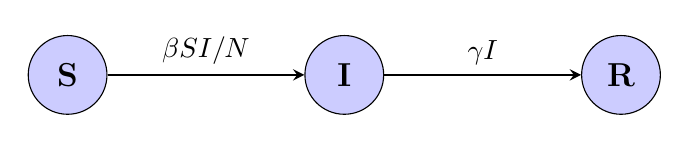
\begin{tikzpicture}[node distance=2.5cm, auto,
    comp/.style={circle, draw, fill=blue!20, minimum size=1cm, font=\large\bfseries},
    arrow/.style={->, thick, >=stealth}]
    
    \node[comp] (S) {S};
    \node[comp, right=of S] (I) {I};
    \node[comp, right=of I] (R) {R};
    
    \draw[arrow] (S) -- node[above] {$\beta SI/N$} (I);
    \draw[arrow] (I) -- node[above] {$\gamma I$} (R);
\end{tikzpicture}
\end{center}

\subsection{SEIR Model}

Adding exposed (latent) compartment:

\begin{center}
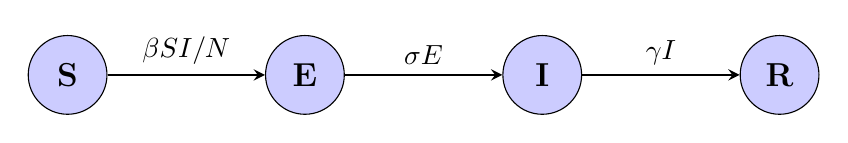
\begin{tikzpicture}[node distance=2cm, auto,
    comp/.style={circle, draw, fill=blue!20, minimum size=1cm, font=\large\bfseries},
    arrow/.style={->, thick, >=stealth}]
    
    \node[comp] (S) {S};
    \node[comp, right=of S] (E) {E};
    \node[comp, right=of E] (I) {I};
    \node[comp, right=of I] (R) {R};
    
    \draw[arrow] (S) -- node[above] {$\beta SI/N$} (E);
    \draw[arrow] (E) -- node[above] {$\sigma E$} (I);
    \draw[arrow] (I) -- node[above] {$\gamma I$} (R);
\end{tikzpicture}
\end{center}

\subsection{SEAIRQHD Model}

A complex model with 8 compartments:

\begin{center}
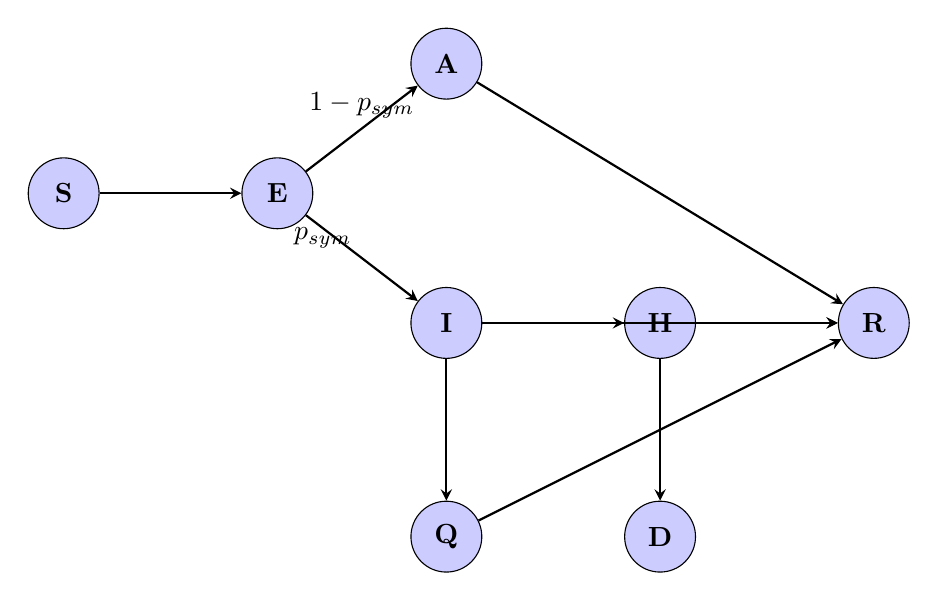
\begin{tikzpicture}[node distance=1.8cm, auto,
    comp/.style={circle, draw, fill=blue!20, minimum size=0.9cm, font=\bfseries},
    arrow/.style={->, thick, >=stealth}]
    
    \node[comp] (S) {S};
    \node[comp, right=of S] (E) {E};
    \node[comp, above right=1cm and 1.5cm of E] (A) {A};
    \node[comp, below right=1cm and 1.5cm of E] (I) {I};
    \node[comp, right=of I] (H) {H};
    \node[comp, below=of I] (Q) {Q};
    \node[comp, right=of H] (R) {R};
    \node[comp, below=of H] (D) {D};
    
    \draw[arrow] (S) -- (E);
    \draw[arrow] (E) -- node[above left] {$p_{sym}$} (I);
    \draw[arrow] (E) -- node[above] {$1-p_{sym}$} (A);
    \draw[arrow] (I) -- (H);
    \draw[arrow] (I) -- (Q);
    \draw[arrow] (I) -- (R);
    \draw[arrow] (A) -- (R);
    \draw[arrow] (H) -- (R);
    \draw[arrow] (H) -- (D);
    \draw[arrow] (Q) -- (R);
\end{tikzpicture}
\end{center}

%==============================================================================
\section{Performance and Validation}
%==============================================================================

\subsection{Model Generation Success Rate}

The constraint-based approach achieves \textbf{100\% valid model generation} across 400 tested configurations:

\begin{center}
\begin{tabular}{@{}lc@{}}
\toprule
\textbf{Validation Check} & \textbf{Pass Rate} \\
\midrule
Population conservation & 100\% \\
No dead-ends & 100\% \\
Infectious pathway & 100\% \\
$R_0 > 0$ & 100\% \\
Numerical stability & 100\% \\
\midrule
\textbf{Overall} & \textbf{100\%} \\
\bottomrule
\end{tabular}
\end{center}

\subsection{Compartment Diversity}

Average statistics from random model generation:

\begin{itemize}[itemsep=0pt]
    \item Average compartments per model: 5.2 (when requesting 5)
    \item Average transitions per model: 6.8
    \item Unique model topologies: 127 (from 400 samples)
\end{itemize}

%==============================================================================
\section{Conclusion}
%==============================================================================

EpiRecipe provides a robust, constraint-based framework for generating diverse compartmental epidemic models. Key achievements include:

\begin{enumerate}[itemsep=0pt]
    \item \textbf{100\% valid model generation} through careful constraint enforcement
    \item \textbf{12 compartment types} covering most epidemiological scenarios
    \item \textbf{20+ transition dynamics} with multiple variants per type
    \item \textbf{Hierarchical parameter sampling} ensuring epidemiological consistency
    \item \textbf{First-class population stratification} with 4 mixing matrix types
    \item \textbf{Web interface} for interactive model exploration
\end{enumerate}

The pipeline is designed to support training of machine learning models for epidemic forecasting by providing a rich, diverse set of synthetic epidemic time series.

%==============================================================================
\appendix
\section{Complete Compartment Dependency Graph}
%==============================================================================

\begin{center}
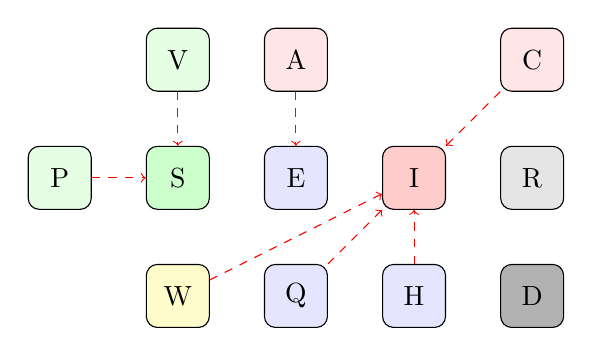
\begin{tikzpicture}[node distance=2cm, auto,
    comp/.style={rectangle, draw, fill=blue!10, minimum size=0.8cm, rounded corners},
    req/.style={->, dashed, red},
    trans/.style={->, thick}]
    
    % Core compartments
    \node[comp, fill=green!20] (S) at (0,0) {S};
    \node[comp, fill=red!20] (I) at (3,0) {I};
    \node[comp] (E) at (1.5,0) {E};
    \node[comp, fill=gray!20] (R) at (4.5,0) {R};
    
    % Extended compartments
    \node[comp, fill=red!10] (A) at (1.5,1.5) {A};
    \node[comp] (H) at (3,-1.5) {H};
    \node[comp, fill=black!30] (D) at (4.5,-1.5) {D};
    \node[comp, fill=green!10] (V) at (0,1.5) {V};
    \node[comp] (Q) at (1.5,-1.5) {Q};
    \node[comp, fill=yellow!20] (W) at (0,-1.5) {W};
    \node[comp, fill=red!10] (C) at (4.5,1.5) {C};
    \node[comp, fill=green!10] (P) at (-1.5,0) {P};
    
    % Dependencies (dashed red)
    \draw[req] (A) -- (E);
    \draw[req] (H) -- (I);
    \draw[req] (W) -- (I);
    \draw[req] (C) -- (I);
    \draw[req] (V) -- (S);
    \draw[req] (P) -- (S);
    \draw[req] (Q) -- (I);
    
\end{tikzpicture}
\end{center}

\textbf{Legend}: Dashed red arrows indicate ``requires inflow from'' dependencies.

\end{document}
